\section{Power Optimised Software Envelope}
\label{sec:pose}

The POSE heuristic partitions the Energy/Runtime plane into areas with differing performance characteristics relative to some initial unoptimised code.
This section introduces the bounds which make up POSE and provides their derivations for the $E^mt^n$ family of metrics.
The only prerequisites of our model are that time and energy consumption can be accurately measured on the target platform.

\begin{figure}
\centering
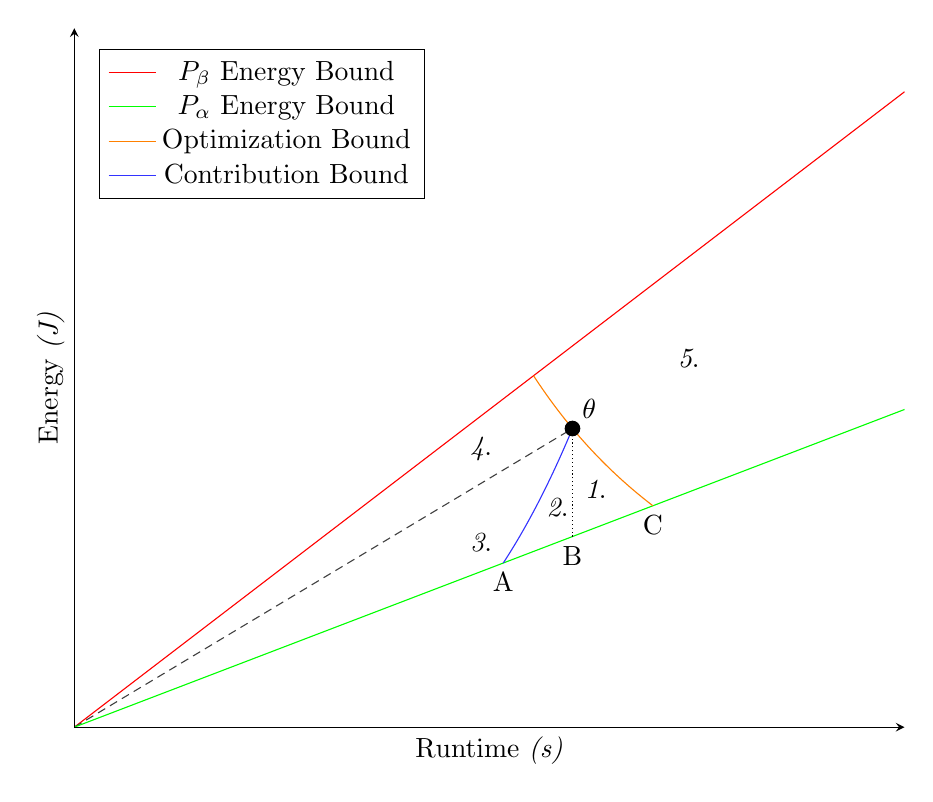
\begin{tikzpicture}
  \begin{axis}[ticks = none, 
    axis on top,
    axis x line=bottom,
    axis y line=left,
  	xlabel={Runtime \emph{(s)}},
    ylabel={Energy \emph{(J)}},    
    xmin=0, xmax=50,
    ymin=0, ymax=3300,
    width=\linewidth,
    legend style={legend pos=north west}
    ]

    %% Model Parameters %%
    \pgfmathsetmacro{\baselinepower}{30} % NOP code
    \pgfmathsetmacro{\rooflinepower}{60}
    \pgfmathsetmacro{\codepower}{47} 
    \pgfmathsetmacro{\codetime}{30}
    % Sadly, pgfplots sucks too much to calculate cube roots
    % These values are calculated with a ruby script in tools
    \pgfmathsetmacro{\anodex}{25.83028}
    \pgfmathsetmacro{\cnodex}{34.84283}
    \pgfmathsetmacro{\tnodex}{27.65477}

    \pgfmathsetmacro{\cnodey}{\cnodex * \baselinepower}
    \pgfmathsetmacro{\anodey}{\anodex * \baselinepower}
 
    %% Intermezzo Values %%
    \pgfmathsetmacro{\codeenergy}{\codepower * \codetime}
    \pgfmathsetmacro{\baselineenergy}{\baselinepower * \codetime}
    \pgfmathsetmacro{\rooflineenergy}{\rooflinepower * \codetime}
    \pgfmathsetmacro{\lowdisplayline}{(2 * \baselinepower + \codepower) / 3}
    \pgfmathsetmacro{\highdisplayline}{(1 * \rooflinepower + 1 * \codepower) / 2}

    % arguments: code power, code time, x - todo, apparently not supposed to do pgfmathparse
    \pgfmathdeclarefunction{metricbound}{3}{%
      \pgfmathparse{((#1 * #2^3) / #3^2)}%
    }
    \pgfmathdeclarefunction{definitionbound}{3}{%
      \pgfmathparse{((#1 / #2^3) * #3^4)}%
    }

    % BETA ROOFLINE BOUND
    \addplot[color=red, domain=\pgfkeysvalueof{/pgfplots/xmin}:\pgfkeysvalueof{/pgfplots/xmax}] {\rooflinepower * x};
    \addlegendentry{$P_{\beta}$ Energy Bound}

    %const power diagonal
    \addplot[color=darkgray, densely dashed, forget plot, %forget plot prevents legend entry
            domain=\pgfkeysvalueof{/pgfplots/xmin}:\codetime] {\codepower * x}; 

    % ALPHA BASELINE BOUND 
    \addplot[color=green, domain=\pgfkeysvalueof{/pgfplots/xmin}:\pgfkeysvalueof{/pgfplots/xmax}] {\baselinepower * x};
    \addlegendentry{$P_{\alpha}$ Energy Bound} 

    \addplot[color=orange, domain=\tnodex:\cnodex] { metricbound(\codepower, \codetime, x)};
    \addlegendentry{Optimization Bound}

    \addplot[color=blue!80, domain=\anodex:\codetime] { definitionbound(\codepower, \codetime, x)};
    \addlegendentry{Contribution Bound}

    % Constant Time, Energy Dashes
    %vertical
    \draw[densely dotted] ({axis cs:\codetime,\baselineenergy}) -- ({axis cs:\codetime,\codeenergy});

    \node[circle,fill,inner sep=2pt] at (axis cs:\codetime,\codeenergy) {};
    \node[above right] at (axis cs:\codetime,\codeenergy) {$\theta$};
    \pgfmathsetmacro{\oneycoord}{\lowdisplayline * 31.4}
    \node at (axis cs:31.4,\oneycoord) {\textit1.};
    \pgfmathsetmacro{\twoycoord}{\lowdisplayline * 29.1}
    \node at (axis cs:29.1,\twoycoord) {\textit2.};
    \pgfmathsetmacro{\threeycoord}{\lowdisplayline * 24.5}
    \node at (axis cs:24.5,\threeycoord) {\textit3.};
    \pgfmathsetmacro{\fourycoord}{\highdisplayline * 24.5}
    \node at (axis cs:24.5,\fourycoord) {\textit4.};
    \pgfmathsetmacro{\fiveycoord}{\codepower * 37}
    \node at (axis cs:37,\fiveycoord) {\textit5.};
    
    \node [below] at ({axis cs:\anodex, \anodey}) {A};
    \node [below] at ({axis cs:\codetime,\baselineenergy}) {B};
    \node [below] at ({axis cs:\cnodex, \cnodey}) {C};
    %\node [below, name intersections={of=metric bound and baseline}] at (intersection-1) {C};


 \end{axis}
\end{tikzpicture}

\caption{$E^1t^2$ Power Optimised Software Envelope}
\label{fig:technique}
\end{figure}

\subsection{Feasible Performance Envelope}
POSE is built around the concept of a \emph{Feasible Performance Envelope}.
We construct this by plotting lines of gradient $P_{max}$ and $P_{min}$ in \autoref{fig:technique}.
These values represent the maximum and minimum rates of power consumption which can occur during normal operation of the target platform.
The $\langle Runtime, Energy\rangle$ costs incurred by running any given code $\theta$ under similar conditions must be represented somewhere within this envelope.

\subsection{Optimisation Bound}
To constrain our search space further we consider the metric we wish to reduce.

\begin{definition}
For logically equivalent codes $\theta$ and $\lambda$, the transformation ${\theta \to \lambda}$ is a valid optimisation with respect to cost metric $M$ if and only if ${M(\lambda) < M(\theta)}$.
\label{def:optimisation}
\end{definition}

We plot a curve passing through $\theta$ linking all points where ${M(\lambda) = M(\theta)}$. By \autoref{def:optimisation} any optimised versions of $\theta$ must exist below this bound.
Naturally the equation for the Optimisation Bound depends on the metric we are optimising for.
\autoref{fig:technique} shows the Optimisation Bound for $E^1t^2$.
The general form of this bound for the $E^mt^n$ family of metrics is derived as follows:
\begin{align}
 {E_\lambda}^m{t_\lambda}^n &= {E_\theta}^m{t_\theta}^n \nonumber \\
 {E_\lambda}^m &= \frac{{E_\theta}^m{t_\theta}^n}{{t_\lambda}^n} \nonumber \\
  E_\lambda &= (\frac{{E_\theta}^m{t_\theta}^n}{{t_\lambda}^n})^\frac{1}{m}
\label{eq:optimisation}
\end{align}

\subsection{Contribution Bound}
Our second bound considers what it means to optimise for reduced power draw.

\begin{definition}
An optimisation $\theta \to \lambda$ with respect to metric $M$ is a power optimisation if the reduction in power draw it delivers is responsible for the majority of the improvement in $M$.
\label{def:poweropt}
\end{definition}

We plot a curve through $\theta$ linking all points for which power and runtime factors contribute to $M$ in the same ratio as our original code.
By \autoref{def:poweropt} any power-optimised versions of $\theta$ must lie below this Contribution Bound.
Again the equation for the Contribution Bound depends on the metric chosen. 
\autoref{fig:technique} shows the bound for $E^1t^2$ while the general form for $E^mt^n$ metrics is derived as follows:
\begin{align}
\frac{{P_{\lambda}}^m}{{t_{\lambda}}^{m+n}} &= \frac{{P_{\theta}}^m}{{t_{\theta}}^{m+n}} \nonumber \\
 {P_{\lambda}}^m &= \frac{{P_{\theta}}^m}{{t_{\theta}}^{m+n}} \times {t_\lambda}^{m+n} \nonumber \\ 
 {E_{\lambda}}^m &= \frac{{P_{\theta}}^m}{{t_{\theta}}^{m+n}} \times {t_\lambda}^{m+n+1} \nonumber \\ 
  E_{\lambda} &= (\frac{{P_{\theta}}^m}{{t_{\theta}}^{m+n}} \times {t_\lambda}^{m+n+1})^{\frac{1}{m}} 
\end{align}

It makes sense to use the most appropriate tools while searching for optimisations.
If an optimisation yields dramatic reductions in runtime with only minor reductions in power consumption then it is reasonable to classify it as a runtime optimisation and state that conventional time-based profilers and performance engineering tools are better suited to finding it.
It is the Contribution Bound which enables our model to make this distinction.
\subsection{Optimisation Limit}
The bounds described thus far delineate those areas of the Energy/Runtime plane in which runtime and power optimised versions of a given code may exist.
The final component of POSE is the Optimisation Limit.
This partitions runtime optimisations into those which strictly dominate all power optimisations and those which could potentially be outperformed by them.

This limit is related to the Optimisation Bound and is likewise based on \autoref{eq:optimisation}.
It connects all points with the same value for $M$ as the maximally power-optimised point in our envelope $C$.
All optimisations below this limit strictly dominate any possible power optimisation.

\section{POSE Insights}
\label{sec:insights}
The POSE Model partitions the feasible performance envelope in \autoref{fig:technique} into several areas.
Potential optimisations can be classified according to which of the following labelled areas they appear in:
\begin{multicols}{2}
\begin{enumerate}
\item Strong Runtime Optimisation
\item Weak Runtime Optimisation
\item Power Optimisation
\item Performance Degradation  
\end{enumerate}
\end{multicols}
Area \textbf{1} encompasses all points with a better $M$ value than the best case power optimisation for $\theta$.
Area \textbf{2} encompasses all possible runtime optimisations which have a better performance than $\theta$ in terms of $M$ yet may in turn be beaten by some power optimised version of $\theta$.
Area \textbf{3} contains all optimised versions of $\theta$ for which reductions in $M$ are due primarily or entirely to reductions in power consumption.
Finally, area \textbf{4} corresponds to all codes with strictly worse performance than $\theta$.

A key strength of POSE is that it produces quantitative and actionable insights relating directly to properties of the code.
These insights fall into one of two broad categories, which taken together allow a performance engineer to decide if power optimisation is likely to prove worthwhile.

The first of these categories relates to how much benefit may be offered by power optimisation.
Taking the difference in energy between point $\theta$ and $D$ gives us an upper limit on the amount of energy which can be saved by power optimisation. 
Similarly, the value $M(\theta) - M(C)$ bounds the amount of improvement in our metric we can expect to see from power optimisation.

The second category indicates how much scope a code has for power optimisation.
The difference in runtime between intersect $E$ and $\theta$ represents the maximum increase in runtime we could feasibly trade off to achieve a slower yet more energy efficient code.
The value $t_\theta / t_B$ represents the smallest speed-up which would guarantee a code which outperformed $\theta$ with respect to $M$.
Finally, $t_\theta / t_A$ is the smallest speed-up guaranteed to outperform any power optimised version of $\theta$.

The figures produced by POSE are all upper bounds, and the benefits of power optimisation will be more modest in practice.
Even so, these figures are useful as they allow performance engineers to make informed decisions about where best to focus their optimisation efforts.

\begin{figure}
\centering
\begin{tikzpicture}
  \begin{axis}[ticks = none, 
    axis on top,
    axis x line=bottom,
    axis y line=left,
  	xlabel={Runtime \emph{(s)}},
    ylabel={Energy \emph{(J)}},    
    xmin=0, xmax=50,
    ymin=0, ymax=3300,
    width=\linewidth,
    legend style={legend pos=north west}
    ]

    %% Model Parameters %%
    \pgfmathsetmacro{\baselinepower}{30} % NOP code
    \pgfmathsetmacro{\rooflinepower}{60}
    \pgfmathsetmacro{\codepower}{47} 
    \pgfmathsetmacro{\codetime}{30}




    %% Intermezzo Values %%
    \pgfmathsetmacro{\codeenergy}{\codepower * \codetime}
    \pgfmathsetmacro{\baselineenergy}{\baselinepower * \codetime}
    \pgfmathsetmacro{\rooflineenergy}{\rooflinepower * \codetime}
    \pgfmathsetmacro{\lowdisplayline}{(2 * \baselinepower + \codepower) / 3}
    \pgfmathsetmacro{\highdisplayline}{(1 * \rooflinepower + 1 * \codepower) / 2}

    % arguments: code power, code time, x, n 
    \pgfmathdeclarefunction{metricbound}{4}{%
      \pgfmathparse{((#1 * #2^(#4 + 1)) / #3^#4)}%
    }
    \pgfmathdeclarefunction{definitionbound}{4}{%
      \pgfmathparse{((#1 / #2^(#4 + 1)) * #3^(#4 + 2))}%
    }
 
    % BETA ROOFLINE BOUND
    \addplot[color=red, domain=\pgfkeysvalueof{/pgfplots/xmin}:\pgfkeysvalueof{/pgfplots/xmax}] {\rooflinepower * x};
    \addlegendentry{$P_{\beta}$ Energy Bound}

    %const power diagonal
    \addplot[color=darkgray, densely dashed, name path=constpwr, forget plot, %forget plot prevents legend entry
            domain=\pgfkeysvalueof{/pgfplots/xmin}:\codetime] {\codepower * x}; 

    % ALPHA BASELINE BOUND 
    \addplot[color=green, name path=basebound, domain=\pgfkeysvalueof{/pgfplots/xmin}:\pgfkeysvalueof{/pgfplots/xmax}] {\baselinepower * x};
    \addlegendentry{$P_{\alpha}$ Energy Bound} 

    % Constant Time vertical dots
    %vertical
    \draw[densely dotted] ({axis cs:\codetime,\baselineenergy}) -- ({axis cs:\codetime,\codeenergy});

    % Sadly, pgfplots sucks too much to calculate cube roots
    % Domain values are calculated with a ruby script in tools

    %% Energy Area %%
    \addplot[name path=energy, draw=none, domain=19.14894:47, forget plot]{ min(definitionbound(\codepower, \codetime, x, 0),metricbound(\codepower, \codetime, x, 0))};
    \addplot[blue!6] fill between[of=energy and basebound];
    \addlegendentry{Energy}

    %% Energy Delay Product Area %% 
    \addplot[name path=edp, draw=none, domain=23.96806:37.54997, forget plot] { min(definitionbound(\codepower, \codetime, x, 1),metricbound(\codepower, \codetime, x, 1))};
    \addplot[blue!13] fill between[of=edp and basebound];
    \addlegendentry{$EDP$}

    %% Energy Delay Squared Product Area ##
    \addplot[name path=edtwop, draw=none, domain=25.83028:34.84283, forget plot] { min(definitionbound(\codepower, \codetime, x, 2),metricbound(\codepower, \codetime, x, 2))};
    \addplot[blue!21] fill between[of=edtwop and basebound];
    \addlegendentry{$ED^2P$}

    %% Energy Delay Cubed Product Area ##
    \addplot[name path=edthreep, draw=none, domain=26.81496:33.56336, forget plot] { min(definitionbound(\codepower, \codetime, x, 3),metricbound(\codepower, \codetime, x, 3))};
    \addplot[blue!35] fill between[of=edthreep and basebound];
    \addlegendentry{$ED^3P$}




     \node[circle,fill,inner sep=2pt] at (axis cs:\codetime,\codeenergy) {};
    \node[above right] at (axis cs:\codetime,\codeenergy) {$\theta$};
  \end{axis}
\end{tikzpicture}

\caption{POSE for Different Metrics}
\label{fig:multimetric-technique}
\end{figure}

It is worth restating that POSE is a metric-agnostic heuristic. \autoref{fig:multimetric-technique} shows how the POSE heuristic varies with choice of metric using Energy ($E^1t^0$) and Energy Delay Squared Product $E^1t^2$ as examples. POSE offers the same insights regardless of the metric chosen.

